\documentclass[13pt,a4paper]{report}
\usepackage[margin=0.6in]{geometry}
\usepackage{fancybox}
\usepackage[utf8]{inputenc}
\usepackage[vietnamese,main=english]{babel}
\usepackage{multicol}
\usepackage{tabularx}
\usepackage{lmodern}
\usepackage{indentfirst}
\usepackage{float}
\usepackage{enumitem}
\usepackage{afterpage}
\usepackage[super]{nth}
\usepackage{titlesec}
\usepackage{bigdelim}
\usepackage[titles]{tocloft}
\usepackage{makecell}
\usepackage{arydshln}
\usepackage{perpage} %the perpage package
\usepackage{graphicx}
\usepackage{caption}
\usepackage{minted}
\usepackage{gensymb}
\usepackage{tikz}
\usepackage{circuitikz}
\usepackage{pgfplots}
\usepackage{cancel}
\usepackage{xurl}
\usepackage[bottom]{footmisc}
\usepackage[font=footnotesize,labelfont={scriptsize}]{subfig}
\usepackage{wrapfig}
\usepackage{latexsym,amssymb,amsmath}
%\usepackage{algpseudocode}
\usepackage{tocvsec2}
\usepackage{fancyref}
\usepackage{bookmark}
\usepackage{hyperref}
\usepackage[nameinlink,noabbrev]{cleveref}

\newcolumntype{Y}{>{\centering\arraybackslash}X}

\PassOptionsToPackage{hyphens}{url}

\makeatletter
\pgfcircdeclarebipole{}{\ctikzvalof{bipoles/vsourceam/height}}{vsourceAM}{\ctikzvalof{bipoles/vsourceam/height}}{\ctikzvalof{bipoles/vsourceam/width}}{%
  \pgfsetlinewidth{\pgfkeysvalueof{/tikz/circuitikz/bipoles/thickness}\pgfstartlinewidth}
   \pgfpathellipse{\pgfpointorigin}{\pgfpoint{0}{\pgf@circ@res@up}}{\pgfpoint{\pgf@circ@res@left}{0}}
   \pgfusepath{draw}
   \pgfscope
       \pgftransformxshift{0.6*\ctikzvalof{bipoles/vsourceam/margin}\pgf@circ@res@left}
       \pgftext[rotate=-\pgf@circ@direction]{$+$}
       \pgfusepath{draw}
   \endpgfscope
   \pgfscope
       \pgftransformxshift{0.6*\ctikzvalof{bipoles/vsourceam/margin}\pgf@circ@res@right}
       \pgftext[rotate=-\pgf@circ@direction]{$-$}
       \pgfusepath{draw}
   \endpgfscope
}
\makeatother

\MakePerPage{footnote} %the perpage package command
\usetikzlibrary{shapes,positioning,arrows,calc,automata}

\newcommand*\justify{%
  \fontdimen2\font=0.4em% interword space
  \fontdimen3\font=0.2em% interword stretch
  \fontdimen4\font=0.1em% interword shrink
  \fontdimen7\font=0.1em% extra space
  \hyphenchar\font=`\-% allowing hyphenation
}
\renewcommand\cftchapafterpnum{\vskip-2pt}
\renewcommand\cftsecafterpnum{\vskip-2pt}

\renewcommand{\theequation}{\arabic{equation}}

% FLOW CHART
\tikzstyle{startstop} = [rectangle, rounded corners, minimum width=3cm, minimum height=1cm,text centered, draw=black, fill=red!30]
\tikzstyle{io} = [trapezium, trapezium left angle=70, trapezium right angle=110, minimum width=3cm, minimum height=1cm, text centered, draw=black, fill=blue!30]
\tikzstyle{process} = [rectangle, minimum width=3cm, minimum height=1cm, text centered, draw=black, fill=orange!30, text width=4cm]
\tikzstyle{decision} = [diamond, aspect=2.5, minimum width=3cm, minimum height=1cm, text centered, draw=black, fill=green!30]
\tikzstyle{arrow} = [thick,->,>=stealth]

% CHAPTER FORMAT
\titleformat{\chapter}%[display]
{\bfseries\fontsize{25}{30}\selectfont\raggedright}% Format and size of title text
{\llap{%
    \rule[-6pt]{6cm}{1.18cm}\rule{6pt}{0pt}}% Black box to the left, lowered 6pt. The end rule is a horisontal space.
  \llap{% Number also to the left, on top of the black box.
    \fontsize{22}{44}\selectfont\color{white}\thechapter\rule{10pt}{0pt}}}{0pt}{}{}

\counterwithin{figure}{section}
\renewcommand{\thefigure}{\arabic{chapter}.\arabic{section}.\alph{figure}}

\renewcommand{\thetable}{\arabic{table}}

\renewcommand\labelitemi{$-$}
  
\titleformat{\section}
  {\LARGE\bfseries}{}{}{}
\renewcommand\thesection{\arabic{section}.}
\renewcommand\thesubsection{\arabic{subsection}}
\makeatletter
\renewcommand*\l@section{\@dottedtocline{1}{1.5cm}{2em}}
\renewcommand\section{\@startsection {section}{1}{-1em}%
  {-3.5ex \@plus -1ex \@minus -.2ex}%
  {2.3ex \@plus.2ex}%
  {\normalfont\Large\bfseries}}
\def\sectionmark#1{%
      \markright {\MakeUppercase{#1}}}
\makeatother

\titleformat{\subsection}
  {\normalfont\bfseries}{\thesubsection.}{0.5em}{}
\renewcommand\cftsubsecaftersnum{.} 
\renewcommand\thesubsection{\alph{subsection}}

\addto{\captionsenglish}{%
  \renewcommand{\bibname}{References}
}

%\addtocontents{toc}{\setcounter{tocdepth}{2}}
%\addtocontents{lof}{\vskip -1.6cm}
%\addtocontents{lot}{\vskip -1.6cm}

    
% TOC settings
\renewcommand\cftchapnumwidth{2.8em}
\renewcommand\cftsecnumwidth{3em}
\renewcommand\cftsecindent{3em}
\renewcommand\cftsubsecindent{5em}
\renewcommand\thechapter{\Roman{chapter}}
    
%\titleformat{\chapter}[display]{\normalfont\huge\bfseries}{}{0pt}{\Huge}
\newcommand{\hsp}{\hspace{20pt}}
%\titleformat{\chapter}[hang]{\Huge\bfseries}{\thechapter\hsp\textcolor{gray75}{|}\hsp}{0pt}{\Huge\bfseries}
\titleformat*{\subsubsection}{\large\bfseries}
%\titlespacing*{\chapter}{0pt}{0pt}{0pt}
    
\newcolumntype{P}[1]{>{\centering\arraybackslash}p{#1}}
\newcolumntype{C}{>{\centering\arraybackslash}p{4em}}
    
\setlist[itemize]{noitemsep, topsep=0pt}
%\AtBeginEnvironment{multicols}{\RaggedRight}

\titlespacing*{\chapter}{0pt}{0pt}{20pt}

\newcommand\Chapter[2]{\chapter
  [#1\text{: }\hfil\hbox{}\protect\linebreak{\itshape#2}]%
  {#1\\[-0.75ex]\Large#2}%
  \markboth{\MakeUppercase{\chaptername\ \thechapter.\ #1}}{}%
}


\def\doubleoverline#1{\overline{\overline{#1}}}

\captionsetup[subfloat]{labelformat=empty}

\begin{document}
%Trang bìa 1
\fontsize{13pt}{18pt}\selectfont
\begin{titlepage}
\thispagestyle{empty}
\thisfancypage{%đóng khung trang này
\setlength{\fboxsep}{0pt}% 8pt là độ dày của đường viền
\fbox}{} % phần nội dung sau là tương tự như đã làm
\

\begin{center}
\begin{large}
HO CHI MINH CITY UNIVERSITY OF TECHNOLOGY $-$ VNU HCMC
\end{large} \\
\begin{large}
OFFICE FOR INTERNATIONAL STUDY PROGRAM
\end{large} \\
\begin{large}
FACULTY OF ELECTRICAL AND ELECTRONIC ENGINEERING
\end{large} \\
\textbf{--------------------  *  --------------------}\\[4cm]
\includegraphics[scale=0.1]{logobk.png}\\[1cm]
{\fontsize{20pt}{1}\selectfont DIGITAL SYSTEMS (LAB)}\\
{\fontsize{20pt}{1}\selectfont EXPERIMENTAL REPORT (PreLab 4)}\\[2.5cm]
\end{center}

\begin{otherlanguage}{vietnamese}
\begin{tabbing}
	\hspace{3.5cm}Lecturer  \ \ \ \ \=: \textbf{\parbox[t]{9cm}{Mr. Nguyễn Tuấn Hùng}}\\
	\hspace{3.5cm}Subject \>: \textbf{\parbox[t]{12cm}{Digital Systems}}\\
	\hspace{3.5cm}Class \>: \textbf{\parbox[t]{9cm}{TT06}}\\
	\hspace{3.5cm}Name \>: \textbf{\parbox[t]{9cm}{
		Lương Triển Thắng}}\\
	\hspace{3.5cm}Student ID \>: \textbf{\parbox[t]{9cm}{
		2051194}}\\[40pt]
\end{tabbing}
\end{otherlanguage}

\vspace{2.25cm}
\begin{center}
{\fontsize{13pt}{1}\selectfont Ho Chi Minh City, \nth{7} June, 2022}
\end{center}
\end{titlepage}

\tableofcontents

\setminted{fontsize=\normalsize}

\setcounter{chapter}{3}

\Chapter{Pre Laboratory 4}{Finite State Machines}

\section{Create state diagram and build the circuit for a finite state machine}
\subsection{Next state table}
\vspace{-0.5cm}
\ctikzset{logic ports=ieee}
\begin{table}[H]
\centering
\begin{tabular}{cc|cccc|cc}
\multicolumn{2}{c|}{\multirow{2}{*}{Present State}}                                                       & \multicolumn{4}{c|}{Next State}                                                                                                                                                                                      & \multicolumn{2}{c}{Output}                                  \\
\multicolumn{2}{c|}{}                                                                                     & \multicolumn{2}{c}{$w=0$}                                                                                  & \multicolumn{2}{c|}{$w=1$}                                                                                  & $w=0$                          & $w=1  $                        \\ \hline
$A$                          & 000000001                                                                    & $B$                          & 000000010                                                                   & $F$                          & 000100000                                                                    & 0                            & 0                            \\
$B$                          & 000000010                                                                    & $C$                          & 000000100                                                                   & $F$                          & 000100000                                                                    & 0                            & 0                            \\
$C$                          & 000000100                                                                    & $D$                          & 000001000                                                                   & $F$                          & 000100000                                                                    & 0                            & 0                            \\
$D$                          & 000001000                                                                    & $E$                          & 000010000                                                                   & $F$                          & 000100000                                                                    & 0                            & 0                            \\
$E$                          & 000010000                                                                    & $E$                          & 000010000                                                                   & $F$                          & 000100000                                                                    & 1                            & 0                            \\
$F$                          & 000100000                                                                    & $B$                          & 000000010                                                                   & $G$                          & 001000000                                                                    & 0                            & 0                            \\
$G$                          & 001000000                                                                    & $B$                          & 000000010                                                                   & $H$                          & 010000000                                                                    & 0                            & 0                            \\
$H$                          & 010000000                                                                    & $B$                          & 000000010                                                                   & $I$                          & 100000000                                                                    & 0                            & 0                            \\
$I$                          & 100000000                                                                    & $B$                          & 000000010                                                                   & $I$                          & 100000000                                                                    & 0                            & 1                            \\
\multicolumn{1}{l}{Others} & \multicolumn{1}{c|}{$\times$} & \multicolumn{1}{l}{Others} & \multicolumn{1}{c}{$\times$} & \multicolumn{1}{l}{Others} & \multicolumn{1}{c|}{$\times$} & \multicolumn{1}{c}{$\times$} & \multicolumn{1}{c}{$\times$}
\end{tabular}
\end{table}

\subsection{Functions for flip-flops}
\begin{table}[H]
\centering
\scalebox{1.2}{
\begin{tabular}{lll}
$D_8 = w(Q_7 + Q_8)$ & $D_5 = \overline Q_5 \overline Q_6 \overline Q_7 \overline Q_8 w$ & $D_2 = Q_1 \overline w$                                                     \\
$D_7 = Q_6 w$        & $D_4 = \overline w (Q_3 + Q_4)$                                   & $D_1 = \overline Q_1 \overline Q_2 \overline Q_3 \overline Q_4 \overline w$ \\
$D_6 = Q_5 w$        & $D_3 = Q_2 \overline w$                                           & $z = \overline Q_4 + \overline Q_8$                                        
\end{tabular}
}
\end{table}

\subsection{Circuit diagram}
\begin{figure}[H]
\centering
\scalebox{0.8}{
\begin{circuitikz}
\draw
	(8,0) node[flipflop D, scale=0.5] (D1) {}
	(8,-1.5) node[flipflop D, scale=0.5] (D2) {}
	(8,-3) node[flipflop D, scale=0.5] (D3) {}
	(8,-4.5) node[flipflop D, scale=0.5] (D4){}
	(8,-6) node[flipflop D, scale=0.5] (D5){}
	(8,-7.5) node[flipflop D, scale=0.5] (D6){}
	(8,-9) node[flipflop D, scale=0.5] (D7){}
	(8,-10.5) node[flipflop D, scale=0.5] (D8){}


	(0,0) node[or port] (or0){}
	(0,-1.5) node[and port] (and2){}
	(0,-3) node[and port] (and3){}
	(0,-4.5) node[and port, number inputs=5] (and-1){}
	(0,-6) node[or port] (or2){}
	(0,-7.5) node[and port] (and4){}
	(0,-9) node[and port] (and5){}
	(0,-10.5) node[and port, number inputs=5] (and6){}
	(0,-12) node[or port] (orz){}
	
	(4, 0) node[and port](and1){}
	(4, -6) node[and port] (and8) {}
  ;
  
\draw
	(and1.out) |- (D1.pin 1)
	(and2.out) |- (D2.pin 1)
	(and3.out) |- (D3.pin 1)
	(and-1.out) |- (D4.pin 1)
	(and8.out) |- (D5.pin 1)
	(and4.out) |- (D6.pin 1)
	(and5.out) |- (D7.pin 1)
	(and6.out) |- (D8.pin 1)
	
	(D1.pin 6) -- ++(1,0) node[anchor=west] {$Q_8$}
	(D2.pin 6) -- ++(1,0) node[anchor=west] {$Q_7$}
	(D3.pin 6) -- ++(1,0) node[anchor=west] {$Q_6$}
	(D4.pin 6) -- ++(1,0) node[anchor=west] {$Q_5$}
	(D5.pin 6) -- ++(1,0) node[anchor=west] {$Q_4$}
	(D6.pin 6) -- ++(1,0) node[anchor=west] {$Q_3$}
	(D7.pin 6) -- ++(1,0) node[anchor=west] {$Q_2$}
	(D8.pin 6) -- ++(1,0) node[anchor=west] {$Q_1$}

	(or0.in 1) -- ++(-2,0) node[anchor=east]{$Q_7$}
	(or0.in 2) -- ++(-2,0) node[anchor=east]{$Q_8$}
	(or0.out) |- (and1.in 1)
	(and1.in 2) -- ++(-1,0) node[anchor=east]{$w$}
	
	(and2.in 1) -- ++(-2,0) node[anchor=east]{$Q_6$}
	(and2.in 2) -- ++(-2,0) node[anchor=east]{$w$}
	(and3.in 1) -- ++(-2,0) node[anchor=east]{$Q_5$}
	(and3.in 2) -- ++(-2,0) node[anchor=east]{$w$}
	
	(and-1.in 1) -- ++(-0.5,0) node[anchor=east]{\footnotesize $\overline Q_5$}
	(and-1.in 2) -- ++(-1,0) node[anchor=east]{\footnotesize $\overline Q_6$}
	(and-1.in 3) -- ++(-1.5,0) node[anchor=east]{\footnotesize $\overline Q_7$}
	(and-1.in 4) -- ++(-2,0) node[anchor=east]{\footnotesize $\overline Q_8$}
	(and-1.in 5) -- ++(-2.5,0) node[anchor=east]{\footnotesize $w$}
	
	(or2.in 1) -- ++(-2,0) node[anchor=east]{$Q_3$}
	(or2.in 2) -- ++(-2,0) node[anchor=east]{$Q_4$}
	(or2.out) |- (and8.in 1)
	(and8.in 2) -- ++(-1,0) node[anchor=east]{$\overline w$}
	
	(and4.in 1) -- ++(-2,0) node[anchor=east]{$Q_2$}
	(and4.in 2) -- ++(-2,0) node[anchor=east]{$\overline w$}
	(and5.in 1) -- ++(-2,0) node[anchor=east]{$Q_1$}
	(and5.in 2) -- ++(-2,0) node[anchor=east]{$\overline w$}
	
	
	(and6.in 1) -- ++(-0.5,0) node[anchor=east]{\footnotesize $\overline Q_1$}
	(and6.in 2) -- ++(-1,0) node[anchor=east]{\footnotesize $\overline Q_2$}
	(and6.in 3) -- ++(-1.5,0) node[anchor=east]{\footnotesize $\overline Q_3$}
	(and6.in 4) -- ++(-2,0) node[anchor=east]{\footnotesize $\overline Q_4$}
	(and6.in 5) -- ++(-2.5,0) node[anchor=east]{\footnotesize $\overline w$}
	
	(orz.in 1) -- ++(-2,0) node[anchor=east]{$Q_4$}
	(orz.in 2) -- ++(-2,0) node[anchor=east]{$Q_8$}
	(orz.out) -- ++(9,0) node[anchor=west]{$z$}
	
	(D8.pin 3) -| ++(-1,12) node[anchor=south] {CLK}
	(D1.pin 3) -- ++(-1,0) node[circ]{}
	(D2.pin 3) -- ++(-1,0) node[circ]{}
	(D3.pin 3) -- ++(-1,0) node[circ]{}
	(D4.pin 3) -- ++(-1,0) node[circ]{}
	(D5.pin 3) -- ++(-1,0) node[circ]{}
	(D6.pin 3) -- ++(-1,0) node[circ]{}
	(D7.pin 3) -- ++(-1,0) node[circ]{}
;
\end{circuitikz}
}
\end{figure}


\section{Describe FSM using VHDL behavioral expressions}
\subsubsection{Exc2.vhd}
\begin{minted}{vhdl}
LIBRARY ieee;
USE ieee.std_logic_1164.ALL;
ENTITY Exc2 IS PORT (
	w, clk, rst : IN STD_LOGIC;
	x : OUT STD_LOGIC
);
END Exc2;

ARCHITECTURE Behavior OF Exc2 IS
	TYPE State_type IS (A, B, C, D, E, F, G, H, I);
	ATTRIBUTE syn_encoding : STRING;
	ATTRIBUTE syn_encoding OF State_type : TYPE IS "0000 0001 0010 0011 0100 0101 0110 0111 1000";

	SIGNAL y_Q, Y_D : State_type;
BEGIN
	PROCESS (w, y_D)
	BEGIN
		CASE y_D IS
			WHEN A =>
				IF (w = '0') THEN 
					y_Q <= B;
				ELSE
					y_Q <= F;
				END IF;

			WHEN B =>
				IF (w = '0') THEN
					y_Q <= C;
				ELSE
					y_Q <= F;
				END IF;

			WHEN C =>
				IF (w = '0') THEN
					y_Q <= D;
				ELSE
					y_Q <= F;
				END IF;

			WHEN D =>
				IF (w = '0') THEN
					y_Q <= E;
				ELSE
					y_Q <= F;
				END IF;

			WHEN E =>
				IF (w = '0') THEN
					y_Q <= E;
				ELSE
					y_Q <= F;
				END IF;

				-------------------------
			WHEN F =>
				IF (w = '1') THEN
					y_Q <= G;
				ELSE
					y_Q <= B;
				END IF;

			WHEN G =>
				IF (w = '1') THEN
					y_Q <= H;
				ELSE
					y_Q <= B;
				END IF;

			WHEN H =>
				IF (w = '1') THEN
					y_Q <= I;
				ELSE
					y_Q <= B;
				END IF;

			WHEN I =>
				IF (w = '1') THEN
					y_Q <= I;
				ELSE
					y_Q <= B;
				END IF;
		END CASE;
	END PROCESS;
	x <= '1' WHEN y_D = E OR y_D = I ELSE '0';

	PROCESS (clk, rst)
	BEGIN
		IF rst = '1' THEN
			Y_D <= A;
		ELSE
			IF rising_edge(clk) THEN
				y_D <= y_Q;
			END IF;
		END IF;
	END PROCESS;
END Behavior;
\end{minted}

\section{Implement a shift register}
\subsection{Code}
\subsubsection{Exc3.vhd}
\begin{minted}{vhdl}
LIBRARY ieee;
USE ieee.std_logic_1164.ALL;
USE ieee.numeric_std.ALL;

ENTITY Exc3 IS
	PORT (
		clk, inp, rst : IN STD_LOGIC;    -- rst: active low
		L : OUT STD_LOGIC_VECTOR(0 TO 3)
	);
END Exc3;

ARCHITECTURE arch OF Exc3 IS
	SIGNAL q : STD_LOGIC_VECTOR(0 TO 3);
	COMPONENT DFFn IS
		PORT (
			Din, DClk, DprsN, DclrN, Den : IN STD_LOGIC; -- clr and prs are active low.
			DQ : OUT STD_LOGIC);
	END COMPONENT;
BEGIN
	DFF0 : DFFn PORT MAP(
		Din => inp, DClk => clk, DprsN => '1',
		DclrN => rst, Den => '1', DQ => q(0));
	gen : FOR i IN 1 TO 3 GENERATE
		DFFs : DFFn PORT MAP(
			Din => q(i - 1), DClk => clk, DprsN => '1',
			DclrN => rst, Den => '1', DQ => q(i));
	END GENERATE;
	L <= q;
END ARCHITECTURE;
\end{minted}

\subsection{Waveform}
\begin{figure}[H]
\centering
\includegraphics[scale=0.6]{images/Exc3_waveform.png}
\end{figure}

\subsection{Result of RTL viewer}
\begin{figure}[H]
\centering
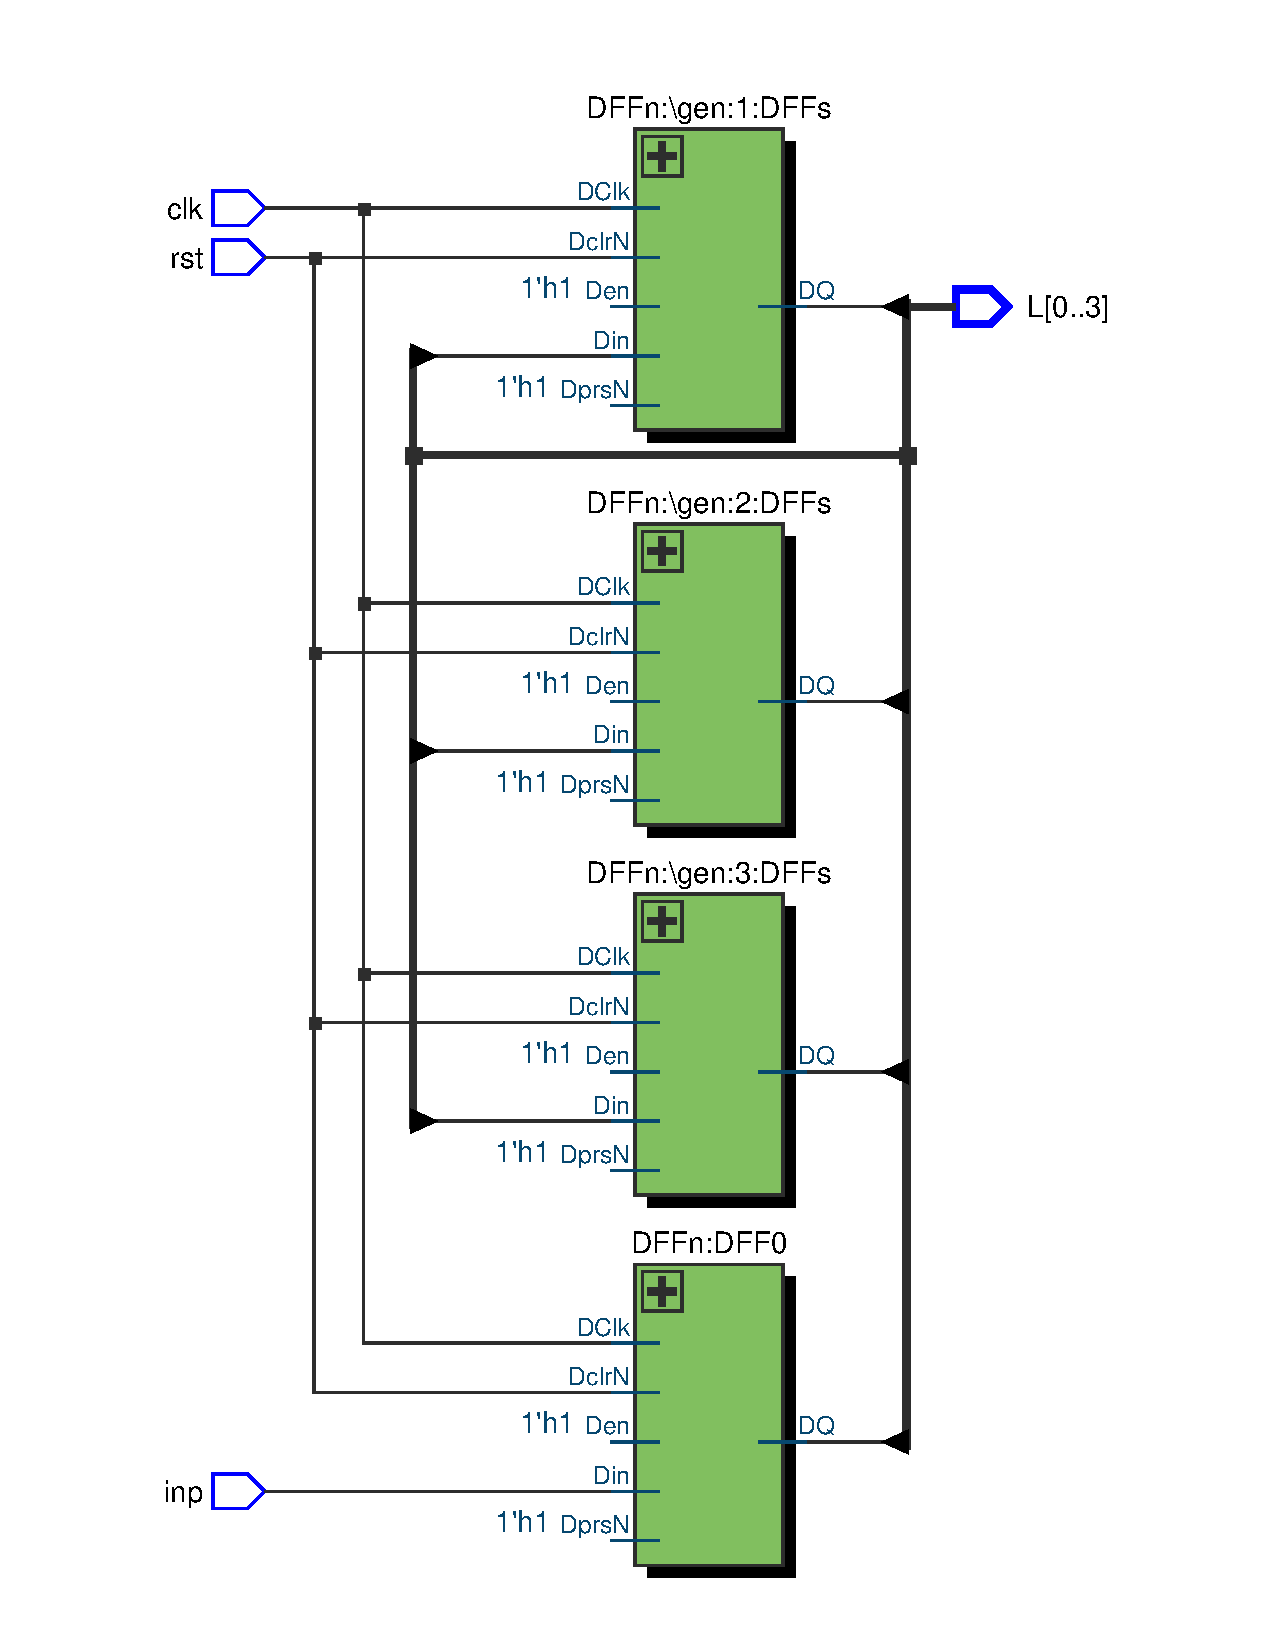
\includegraphics[scale=0.5, clip, trim={0cm 1cm 0cm 1cm}]{images/Exc3_RTL.pdf}
\end{figure}

\section{Implement a periodic signal}
\subsection{Code}
\subsubsection{Exc4.vhd}
\begin{minted}{vhdl}
LIBRARY ieee;
USE ieee.std_logic_1164.ALL;
USE ieee.numeric_std.ALL;

ENTITY Exc4 IS
    GENERIC (rate : INTEGER); -- rate = oldFreq / newFreq
    PORT (
        Clk : IN STD_LOGIC;
        clkout : OUT STD_LOGIC;
        nRst : IN STD_LOGIC -- Negative reset
    );
END ENTITY;

ARCHITECTURE rtl OF Exc4 IS
    -- Signal for counting clock periods
    SIGNAL Ticks : INTEGER := 0;
    SIGNAL clkt : STD_LOGIC := '0';

BEGIN
    clkout <= clkt;
    PROCESS (Clk) IS
    BEGIN
        IF rising_edge(Clk) THEN
            -- If the negative reset signal is active
            IF nRst = '0' THEN
                Ticks <= 0;
            ELSE
                IF Ticks = (rate / 2) - 1 THEN
                    Ticks <= 0;
                    clkt <= NOT (clkt);
                ELSE
                    Ticks <= Ticks + 1;
                END IF;
            END IF;
        END IF;
    END PROCESS;

END ARCHITECTURE;
\end{minted}

\subsubsection{Exc4\_tb.vhd}
\begin{minted}{vhdl}
LIBRARY ieee;
USE ieee.std_logic_1164.ALL;
USE ieee.numeric_std.ALL;

ENTITY Exc4_tb IS
END ENTITY;

ARCHITECTURE sim OF Exc4_tb IS

    -- We're slowing down the clock to speed up simulation time
    CONSTANT ClockFrequencyHz : INTEGER := 10; -- 10 Hz; 50 MHz or 25 MHz for the clock on DE10
    CONSTANT ClockPeriod : TIME := 1000 ms / ClockFrequencyHz;

    SIGNAL Clk : STD_LOGIC := '1';
    SIGNAL nRst : STD_LOGIC := '1';
    SIGNAL clkout : STD_LOGIC;

BEGIN

    -- The Device Under Test (DUT)
    CD : ENTITY work.Exc4(rtl)
        GENERIC MAP(rate => 10) 
        PORT MAP(
            Clk => Clk,
            nRst => nRst,
            clkout => clkout);

    -- Process for generating the clock
    Clk <= NOT Clk AFTER ClockPeriod / 2;

END ARCHITECTURE;
\end{minted}

\subsection{Waveform}
\begin{figure}[H]
\centering
\includegraphics[scale=0.6]{images/Exc4_waveform.png}
\end{figure}

\subsection{Result of RTL viewer}
\begin{figure}[H]
\centering
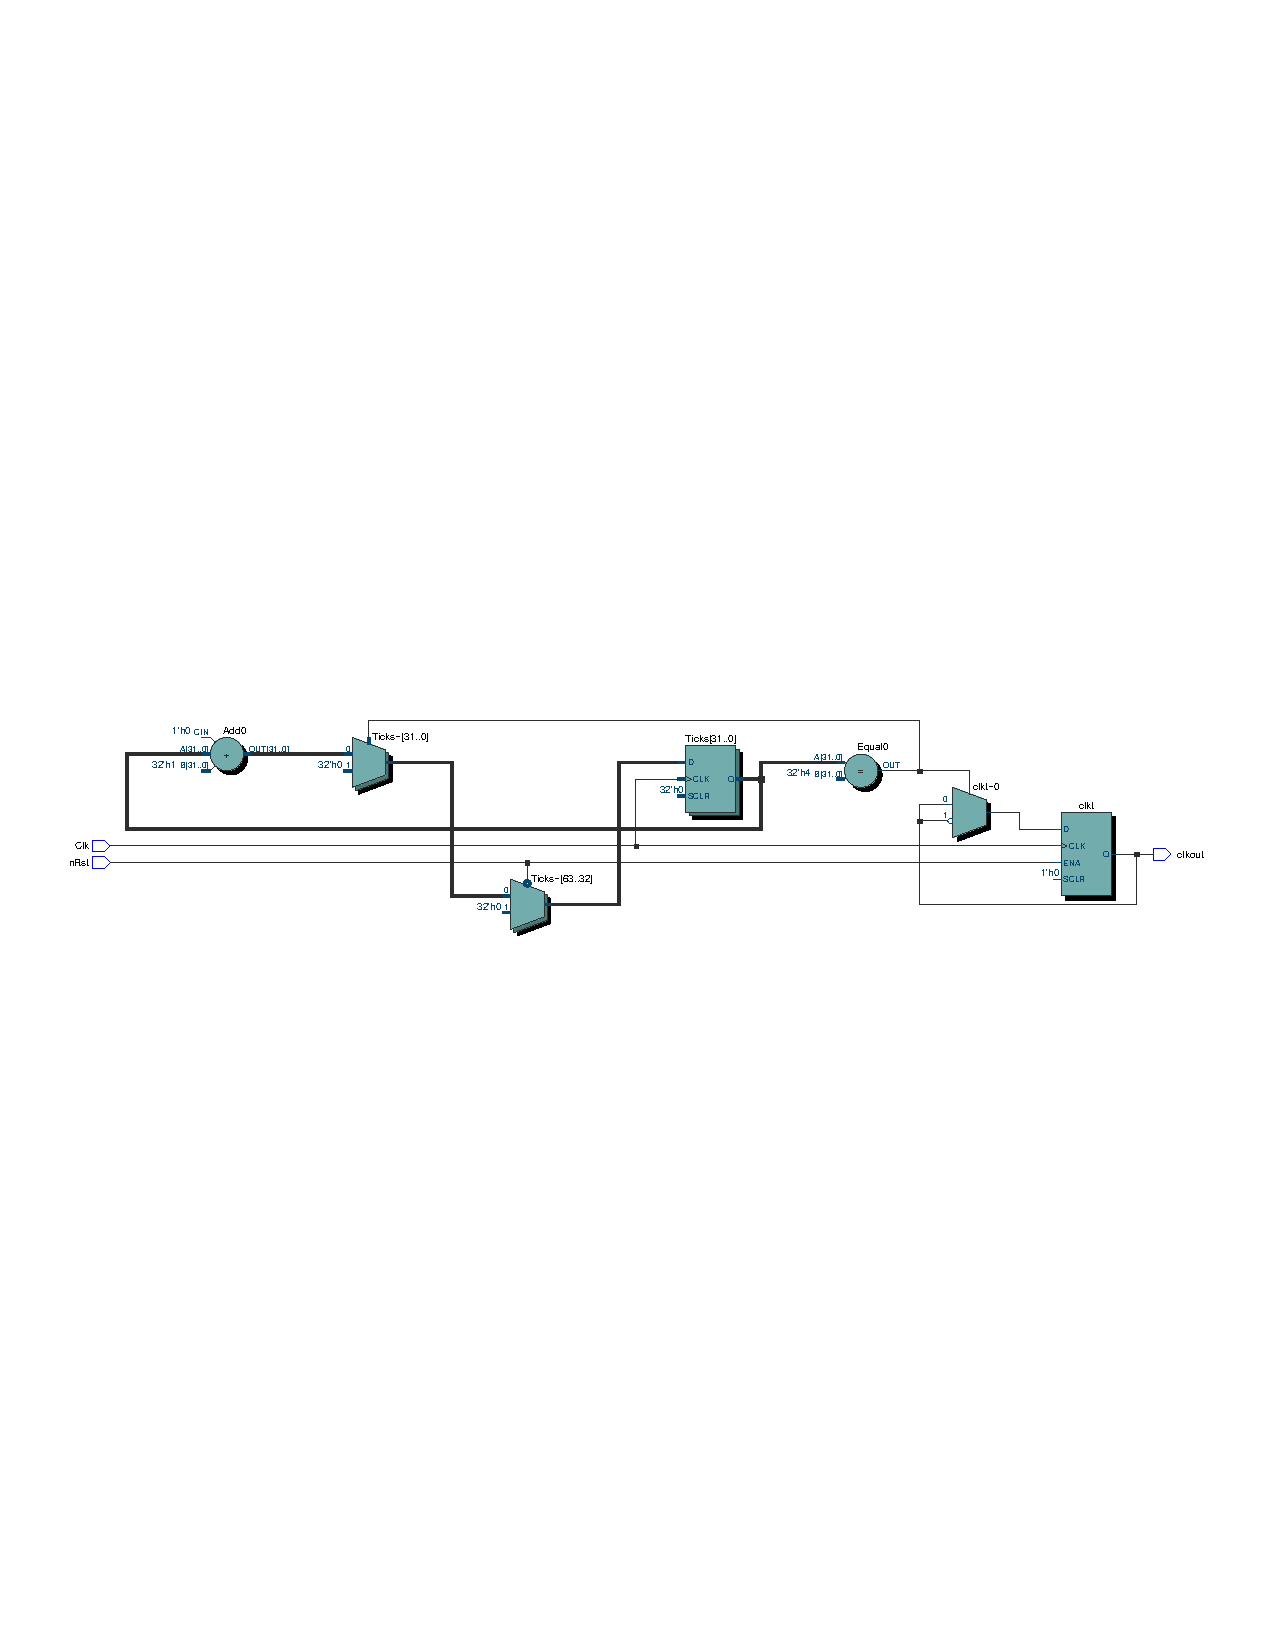
\includegraphics[scale=0.8, clip, trim={0cm 12cm 0cm 12cm}]{images/Exc4_RTL.pdf}
\end{figure}

\section{Know how to implement a digital circuit using an FSM}
In this exercise, I modifed the circuit, so when there is a dot, LED will on for 0.25 second; if there is a dash, LED will on for 1 second.

\tikzset{
->, % makes the edges directed
>=stealth', % makes the arrow heads bold
node distance=5cm, % specifies the minimum distance between two nodes. Change if necessary.
every state/.style={thick, fill=gray!10}, % sets the properties for each ’state’ node
initial text=$ $, % sets the text that appears on the start arrow
}

\subsection{FSM diagram}
\begin{figure}[H]
\centering
\scalebox{0.8}{
\begin{tikzpicture}
\node[state, initial] (idle) {idle};
\node[state, right of=idle] (store) {store};
\node[state, right of=store] (shift) {shift};
\node[state, right of=shift] (setT) {\makecell{Set\\ wait time}};
\node[state, below of=setT] (wait) {wait};
\node[state, left of=wait] (dec) {\makecell{Decrease\\ size}};
\node[state, left of=dec] (check) {\makecell{Check\\ size}};

\draw (idle) edge[loop above] node{btn = 0} (idle)
(idle) edge[above] node{btn = 1} (store)
(store) edge[above] node{} (shift)
(shift) edge[above] node{shifted bit} (setT)
(setT) edge[right] node{ticksToWait} (wait)
(wait) edge[loop below] node{ticks $<$ ticksToWait} (wait)
(wait) edge[above] node{ticks = ticksToWait} (dec)
(dec) edge[above] node{} (check)
(check) edge[left] node{size $>$ 0} (shift)
(check) edge[left] node{size = 0} (idle)
;
\end{tikzpicture}
}
\end{figure}

\subsection{Details}
\begin{itemize}
\item {\bf Idle:} In this state, the circuit waits for user pressing the button.
\item {\bf Store:} The circuit will store morse code and morse length according to the SW[2:0].
\item {\bf Shift:} The circuit shift the bit array to the right.
\item {\bf Set wait time:}
\begin{itemize}
\item[$+$] If shifted \texttt{bit} = 0 (dot), set wait time = 0.25s.
\item[$+$] If shifted \texttt{bit} = 1 (dash), set wait time = 1s.
\end{itemize}

\item {\bf Wait:} The circuit will count \texttt{ticks} until \texttt{ticks = ticksToWait}.
\item {\bf Decrease size:} Decrease size of morse length.
\item {\bf Check size:}
\begin{itemize}
\item[$+$] If \texttt{size} = 0, return to idle state.
\item[$+$] If \texttt{size} $>$ 0, return to shift state.
\end{itemize}
\end{itemize}

\subsection{Expected waveform}
\begin{figure}[H]
\centering
\includegraphics[scale=0.35]{images/Exc5_waveform.png}
\end{figure}
\end{document}